%!TEX program = xelatex
%!TEX options = -shell-escape -8bit
\documentclass[9pt,dvipsnames]{beamer}

\usepackage{amsmath}
\usepackage{amsthm}
\usepackage{amssymb}
\usepackage{arevtext,arevmath}  % should be before fontspec
\SetSymbolFont{largesymbols}{normal}{OMX}{iwona}{m}{n}
\usepackage{mathtools}

\usepackage[no-math,cm-default]{fontspec}
\usepackage[indentfirst]{xeCJK}
\usepackage{comment}
\usepackage{verbatim}
\usepackage{indentfirst}
\usepackage{syntonly}
\usepackage{fancyhdr}
\usepackage{xcolor}
\usepackage{graphicx}
%\usepackage{paralist}
\usepackage{beamerthemesplit}
% \usepackage{euler}
\usepackage{ulem}
% \usepackage{listings}
\usepackage{minted}
\usepackage{zhspacing}
\usepackage{booktabs}
\usepackage{multirow}
\usepackage{supertabular}
\usepackage{nameref}


\usetheme{Berlin}
\usecolortheme{beaver}
\usefonttheme[onlymath]{serif}
\CJKsetecglue{}
% \usefonttheme{professionalfonts}

% \defaultfontfeatures{Mapping=tex-text}
% \zhspacing
% \newfontfamily\zhfont[BoldFont=PingFang SC Semibold]{PingFang SC Light}
\setCJKmainfont[BoldFont={PingFang SC Semibold},ItalicFont={Adobe Fangsong Std}]{PingFang SC Light}
\setmonofont[Scale=1]{Fira Mono}
% \XeTeXlinebreaklocale "zh"
% \XeTeXlinebreakskip = 0pt plus 1pt

% \lstset{language=C++,
%     extendedchars=false,
%     basicstyle=\ttfamily\footnotesize,
%     keywordstyle=\bfseries\color{blue},
%     identifierstyle=\color{blue!60!black},
%     commentstyle=\itshape\color{gray},
%     escapeinside=`'}
\setminted[c++]{
	baselinestretch=0.8,
	breaklines=true,
	frame=lines,
	gobble=1,
	obeytabs,
	stripnl=true,
	tabsize=2
}

\setlength{\parindent}{2em}
\setlength{\baselineskip}{1.3\baselineskip}
%\linespread{1.3}

\setbeamercolor{math text}{fg=black}
\setbeamertemplate{qed symbol}{$\square$}
\setbeamerfont{headline}{size=\fontsize{7pt}{\baselineskip}}
\setbeamerfont{frametitle}{series=\bfseries,size=\fontsize{14pt}{\baselineskip}}
\setbeamerfont{footline}{size=\fontsize{7pt}{\baselineskip}}
\setbeamerfont{title}{series=\bfseries,size=\fontsize{18pt}{\baselineskip}}
\setbeamerfont{subtitle}{series=\bfseries,size=\fontsize{12pt}{\baselineskip}}


\newcommand{\scaledmath}[2][1.5]{\scalebox{#1}[1]{$#2$}}
\renewcommand{\det}[1]{\vert{#1}\vert}
\renewcommand{\d}{\,\mathrm{d}}


\title{数学知识}
\subtitle{线性代数、概率与期望}
\author{清华大学~~胡泽聪}
\date{}

\begin{document}

\maketitle

%\setcounter{tocdepth}{1}
\begin{frame}
	\frametitle{目录}
	\tableofcontents[hideallsubsections]
\end{frame}

\section{线性代数}
\subsection{简介}
\begin{frame}
	\frametitle{知识点列表}
	\begin{enumerate}
		\item 矩阵与矩阵乘法
		\item 矩阵乘法的应用
		\item 行列式、初等行变换
		\item 高斯消元与方程组求解
		\item 行列式的应用:生成树计数
	\end{enumerate}
\end{frame}

\subsection{矩阵与矩阵乘法}
\begin{frame}
	\frametitle{矩阵}
	由$n\times m$个数排成$n$行$m$列的矩形数表:
	\[ \left[\begin{matrix}
		a_{11} & a_{12} & \cdots & a_{1m} \\
		a_{21} & a_{22} & \cdots & a_{2m} \\
		\vdots & \vdots & \ddots & \vdots \\
		a_{n1} & a_{n2} & \cdots & a_{nm} \\
	\end{matrix}\right] \]
	称为一个$n\times m$的矩阵,通常记作$\mathbf{A}$,其中$a_{ij}$为第$i$列第$j$行的元素。

	我们用下面的写法表示:矩阵$\mathbf{A}$由$n\times m$的二维数组$a$构成:
	\[ \mathbf{A}=(a_{ij})_{n\times m} \]
\end{frame}
\begin{frame}
	\frametitle{矩阵乘法}
	设有两个矩阵:$\mathbf{A}=(a_{ij})_{n\times m}$、$\mathbf{B}=(b_{ij})_{m\times r}$。令矩阵$\mathbf{C}$为其乘积$\mathbf{AB}$,那么$\mathbf{C}=(c_{ij})_{n\times r}$,其中:
	\[ c_{ij} = \sum_{k=1}^{m} a_{ik}b_{kj} = a_{i1}b_{1j}+a_{i2}b_{2j}+\cdots+a_{im}b_{mj} \]
\end{frame}
\begin{frame}
	\frametitle{矩阵乘法}
	参考下面的图示:
	\begin{center}
		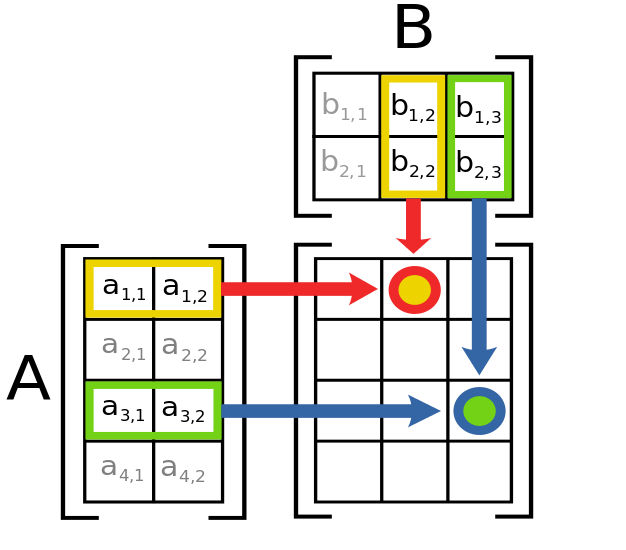
\includegraphics[width=0.5\textwidth]{images/matmul.png}
	\end{center}
\end{frame}
\begin{frame}[fragile]
	\frametitle{矩阵乘法的实现}
	直接实现:
	\begin{minted}{c++}
	struct matrix {
		int n, m, mat[N][N];
	};
	
	matrix matmul(const matrix &a, const matrix &b) {
		matrix c;
		for (int i = 0; i < a.n; ++i)
			for (int j = 0; j < b.m; ++j)
				for (int k = 0; k < a.m; ++k)
					c.mat[i][j] += a.mat[i][k] * b.mat[k][j];
		return c;
	}
	\end{minted}
	复杂度为$O(nmr)$。
\end{frame}
\begin{frame}[fragile]
	\frametitle{矩阵乘法的实现}
	现实中通常需要对模数\texttt{mod}取模:
	\begin{minted}{c++}
		for (int i = 0; i < a.n; ++i)
			for (int j = 0; j < b.m; ++j)
				for (int k = 0; k < a.m; ++k)
					c.mat[i][j] = (c.mat[i][j] + a.mat[i][k] * b.mat[k][j]) % mod;
	\end{minted}
\end{frame}
\begin{frame}[fragile]
	\frametitle{矩阵乘法的实现}
	一个更优的写法是:
	\begin{minted}{c++}
		for (int i = 0; i < a.n; ++i)
			for (int j = 0; j < b.m; ++j) {
				long long tmp = 0LL;
				for (int k = 0; k < a.m; ++k) {
					tmp += a.mat[i][k] * b.mat[k][j];
					if (tmp > 1e18) tmp %= mod;
				}
				c.mat[i][j] = tmp;
			}
	\end{minted}
	\pause
	原理:
	\begin{itemize}
		\item 避免高维数组寻址;
		\item 避免取模:$X,Y\overset{iid}{\scaledmath[2]{\sim}} U[0,2^{31}), \mathbb{E}[XY]=\mathbb{E}[X]\mathbb{E}[Y]=2^{60}\approx \frac{1}{8} 2^{63}$
	\end{itemize}
\end{frame}
\begin{frame}
	\frametitle{矩阵乘法的性质}
	\begin{itemize}
		\item 结合律:$(\mathbf{AB})\mathbf{C} = \mathbf{A}(\mathbf{BC})$ \\
			\hspace{4em}$\mathbf{A}^7=\mathbf{A}^4\times\mathbf{A}^2\times\mathbf{A}^1$
		\item 不满足交换律:$\mathbf{AB}\neq \mathbf{BA}$
	\end{itemize}
\end{frame}
\begin{frame}
	\frametitle{矩阵乘法表示方程组}
	设一个$n$元非齐次线性方程组有$m$个方程如下:
	\[ \arraycolsep=0.5pt
	\left\{\begin{array}{rl}
		a_{11}x_1+a_{12}x_2+\cdots+a_{1n}x_n & = b_1 \\
		a_{21}x_1+a_{22}x_2+\cdots+a_{2n}x_n & = b_2 \\
		\multicolumn{2}{c}{\vdots} \\
		a_{m1}x_1+a_{m2}x_2+\cdots+a_{mn}x_n & = b_m \\
	\end{array}\right. \]

	令$\mathbf{A}=(a_{ij})_{m\times n}$、$\mathbf{x}=(x_i)_{n\times 1}$、$\mathbf{b}=(b_i)_{m\times 1}$,那么方程可以写作
	\[ \mathbf{Ax}=\mathbf{b} \]
	这一写法的好处会在后文中体现。
\end{frame}

\subsection{矩阵乘法的应用}
\begin{frame}
	\frametitle{例题:计算矩阵乘法}
	有两个矩阵$\mathbf{A}=(a_{ij})_{n\times k}$和$\mathbf{B}=(b_{ij})_{k\times n}$,请计算$(\mathbf{AB})^t$。

	$n\leq 1000,\ k\leq 20,\ t<2^{31}$。
\end{frame}
\begin{frame}
	\frametitle{例题:计算矩阵乘法}
	$\mathbf{AB}$为$n\times n$矩阵。利用矩阵快速幂,直接计算的复杂度为$O(n^3\log t)$。\pause

	稍加变形得,$(\mathbf{AB})^t=\mathbf{A}(\mathbf{BA})^{t-1}\mathbf{B}$,而$\mathbf{BA}$是$k\times k$的矩阵。复杂度降为$O(n^2k+k^3\log t)$。\pause

	矩阵乘法虽具有结合律,但\textbf{计算复杂度受计算顺序的影响}。
\end{frame}

\begin{frame}
	\frametitle{例题:求Fibonacci数列}
	Fibonacci数列定义为:
	\[ f_n = \left\{\begin{array}{ll}
		0 & n=0 \\
		1 & n=1 \\
		f_{n-1}+f_{n-2} & n\geq 2 \\
	\end{array}\right. \]
	求其第$n$项。

	$n<2^{63}$。
\end{frame}
\begin{frame}[fragile]
	\frametitle{例题:求Fibonacci数列}
	一种朴素实现如下:
	% \[ \arraycolsep=0.5pt
	% \left\{\begin{array}{rl}
	% 	f_{n-1} & \leftarrow f_{n-1} \\
	% 	f_n & \leftarrow f_{n-1} + f_{n-2}
	% \end{array}\right. \]
	\begin{minted}{c++}
	int fib(int n) {
		int a = 0, b = 1, tmp; // a: f[n-1], b: f[n]
		for (int i = 1; i <= n; ++i)
			tmp = a + b, a = b, b = tmp;
		return a;
	}
	\end{minted}

	\pause 写成矩阵形式:
	\[ \left[\begin{matrix}
		f_{n-1} \\
		f_n \\
	\end{matrix}\right]
	 = \left[\begin{matrix}
		0 & 1 \\
		1 & 1 \\
	\end{matrix}\right]
	\left[\begin{matrix}
		f_{n-2} \\
		f_{n-1} \\
	\end{matrix}\right]
	= \left[\begin{matrix}
		0 & 1 \\
		1 & 1 \\
	\end{matrix}\right]^{n-1}
	\left[\begin{matrix}
		f_0 \\
		f_1 \\
	\end{matrix}\right]\]
\end{frame}

\begin{frame}
	\frametitle{CF341E Wet Sharks and Blocks}
	有$n$个$0\sim 9$的数字,你需要进行$b$次选择,每次从中选出一个数字(可以选择重复的数字)。将选出的数字依次写下,拼成一个大数。求有多少种选法可以使得拼出的数字在模$x$的意义下为$k$。

	$n\leq 50\,000,\ b\leq 10^9,\ 0\leq k<x\leq 100$。
\end{frame}
\begin{frame}
	\frametitle{CF341E Wet Sharks and Blocks}
	考虑动态规划。令$f[i][j]$表示选择$i$个数,在模$x$意义下余$j$的方案数。答案为$f[b][k]$。转移为:
	\[ f[i][j] = \sum_{p=0}^{9}\mathrm{count}(p)\cdot f[i-1][(j-p)/10\bmod{x}] \]
	其中$\mathrm{count}(p)$为数字$p$在$n$个数中的出现次数。\pause

	状态的第二维大小不超过100,转移可以写成矩阵的形式。复杂度为$O(x^3\log b)$。
\end{frame}

\subsection{行列式、初等行变换}
\begin{frame}
	\frametitle{行列式}
	$n$阶行列式是由$n\times n$个数$A=(a_{ij})_{n\times n}$所确定的值,记作:
	\[ \det{\mathbf{A}} = \left\vert\begin{matrix}
		a_{11} & a_{12} & \cdots & a_{1n} \\
		a_{21} & a_{22} & \cdots & a_{2n} \\
		\vdots & \vdots & \ddots & \vdots \\
		a_{n1} & a_{n2} & \cdots & a_{nn} \\
	\end{matrix}\right\vert \]
	也称$\mathbf{A}$的行列式(注意$\mathbf{A}$必须是方阵)。其公式为:
	\[ \sum_{p\in P(n)} (-1)^{\tau(p)} a_{1p_1}a_{2p_2}\cdots a_{np_n} \]
	其中:
	\begin{itemize}
		\item $P(n)$为所有$1\sim n$的排列的集合,$p$取遍所有这样的排列;
		\item $\tau(p)$为排列$p$的逆序对数。
	\end{itemize}
\end{frame}
\begin{frame}
	\frametitle{行列式的性质}
	\begin{enumerate}
		\item 将行和列互换(转置),值不变($\det{\mathbf{A}}=\det{\mathbf{A}^\top}$);\pause
		\item 将一行所有元素同乘以常数$c$,行列式的值乘以$c$;\pause
		\item 交换两行的位置,行列式的值变为相反数;\pause
		\item \textit{(\textbf{初等行变换})}将一行的常数倍加到另一行,行列式的值不变;\pause
		\item \textit{(4的推论)}如果有两行成比例,行列式的值为0;\pause
		\item \textit{(可乘性)}$\det{\mathbf{AB}}=\det{\mathbf{A}}\det{\mathbf{B}}$。
	\end{enumerate}
\end{frame}
\begin{frame}
	\frametitle{初等行变换}
	\textbf{初等行变换}:将一行的常数倍加到另一行,行列式的值不变。
	
	我们想用矩阵形式表示这一变换,即找到一个矩阵,令其左乘另一矩阵,即将该矩阵的第$i$行乘以$k$后加到第$j$行:\pause
	\[ \mathbf{E}_{i,j}^{(k)} = \left[\begin{matrix}
		1                                        \\
		  & \ddots                               \\
		  &        & 1                           \\
		  &        &   & \ddots                  \\
		  &        & k &        & 1              \\
		  &        &   &        &   & \ddots     \\
		  &        &   &        &   &        & 1 \\
	\end{matrix}\right] \]
	即单位阵修改一个元素$e_{ij}=k$。
\end{frame}

\subsection{高斯消元与方程组求解}
\begin{frame}
	\frametitle{非齐次线性方程组}
	非齐次方程组表示为$\mathbf{Ax}=\mathbf{b}$。

	如果$\mathbf{A}$为上三角形式:
	\[ \mathbf{A} = \left[\begin{matrix}
		a_{11} & a_{12} & \cdots & a_{1n} \\
			   & a_{22} & \cdots & a_{2n} \\
			   &        & \ddots & \vdots \\
			   &        &        & a_{nn} \\
	\end{matrix}\right] \]
	那么可以方便倒推求解。
\end{frame}
\begin{frame}
	\frametitle{初等行变换与非齐次线性方程组}
	在等式两侧同时左乘初等行变换矩阵,等式依然成立:
	\[ \big(\mathbf{E}_{i,j}^{(k)}\mathbf{A}\big)\mathbf{x}=\mathbf{E}_{i,j}^{(k)}\mathbf{b} \]

	也即,对矩阵$\mathbf{A}$进行初等行变换,同时令$b_i\leftarrow b_i+k b_j$。

	我们希望通过不断进行这一操作,将矩阵化为上三角形式。
\end{frame}
\begin{frame}
	\frametitle{高斯消元}
	高斯消元方法即这一过程:
	\begin{enumerate}
		\item 输入$n\times n$方阵$\mathbf{A}$和非其次项$\mathbf{b}$。
		\item 枚举每一行$i$,假设$a_{ii}\neq 0$:
			\begin{enumerate}
				\item 对于每个第$j\ (j>i)$行,计算$c=-a_{ji}/a_{ii}$;
				\item 利用初等行变换,将$c$倍的第$i$行加到第$j$行;
				\item 令$b_j\leftarrow b_j+c\cdot b_i$。
			\end{enumerate}
		\item 如果$a_{ii}=0$,那么找到一行$k\ (k>i)$使得$a_{ki}\neq 0$,交换第$i$和第$k$行以及$b_i$和$b_k$,并进行第2步。
		\item 如果在第3步中没有找到非零元素,则方程组有无穷多组解或无解。
	\end{enumerate}
\end{frame}
\begin{frame}
	\frametitle{相关性质与用途}
	\begin{itemize}
		\item 方程$\mathbf{Ax}=\mathbf{b}$有唯一解的充要条件是:$\det{\mathbf{A}}\neq 0$。
		\item 高斯消元法可以将任意矩阵化为上三角矩阵。
		\item 上三角矩阵的行列式为主对角线元素的乘积。
		\item 高斯消元法的复杂度为$O(n^3)$。
	\end{itemize}
\end{frame}

\subsection{行列式的应用}
\begin{frame}
	\frametitle{生成树计数}
	给定一张$n$个节点的无向图$G$,求其生成树方案数。
	\vspace{1em}\pause

	\textbf{基尔霍夫矩阵树定理}(Kirchhoff's matrix tree theorem):
	\begin{enumerate}
		\item 构造图$G$的拉普拉斯矩阵$\mathbf{L}=\mathbf{D}-\mathbf{A}$,其中$\mathbf{D}$是主对角线为各点度数的方阵,$\mathbf{A}$是邻接矩阵;
		\item 任取$r\in[1,n]$,删去$\mathbf{L}$的第$r$行第$r$列,得到其余子式$\mathbf{L}^*_r$;
		\item 求$\mathbf{L}^*_r$的行列式$\det{\mathbf{L}^*_r}$,即为生成树方案数。
	\end{enumerate}
\end{frame}
\begin{frame}
	\frametitle{矩阵树定理:例子}
	以下图为例,图中有4个节点和5条边,共8种生成树。
	\begin{center}
		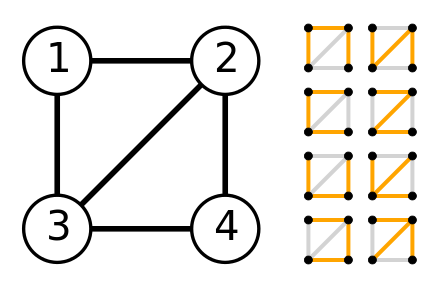
\includegraphics[width=0.3\textwidth]{images/matrixtree.png}
	\end{center}
	\[ \mathmakebox[\textwidth][c]{
		\mathbf{L} = \mathbf{D} - \mathbf{A} = \mathrm{diag}(\{2, 3, 3, 2\}) - \left[\begin{matrix}
			0 & 1 & 1 & 0 \\
			1 & 0 & 1 & 1 \\
			1 & 1 & 0 & 1 \\
			0 & 1 & 1 & 0 \\
		\end{matrix}\right] = \left[\begin{matrix}
			 2 & -1 & -1 &  0 \\
			-1 &  3 & -1 & -1 \\
			-1 & -1 &  3 & -1 \\
			 0 & -1 & -1 &  2 \\
		\end{matrix}\right]
	} \]
	\[ \det{\mathbf{L}^*_1} = \left\vert\begin{matrix}
		 3 & -1 & -1 \\
		-1 &  3 & -1 \\
		-1 & -1 &  2 \\
	\end{matrix}\right\vert = 8 \]
\end{frame}
\begin{frame}
	\frametitle{矩阵树定理:证明}
	设图$G$有$n$个节点和$m$条边,那么其关联矩阵$\mathbf{E}$为$n\times m$的矩阵,其每列代表一条边。如果第$k$条边连接了节点$i$和$j$(不妨设$i<j$),那么$e_{i,k}=1$、$e_{j,k}=-1$。之前的图的关联矩阵为:
	\[ \mathbf{E} = \left[\begin{matrix}
		 1 &  1 &  0 &  0 &  0 \\
		-1 &  0 &  1 &  1 &  0 \\
		 0 & -1 & -1 &  0 &  1 \\
		 0 &  0 &  0 & -1 & -1 \\
	\end{matrix}\right] \]

	不难得出,$\mathbf{L}=\mathbf{EE}^\top$。令$\mathbf{F}$为$\mathbf{E}$删去第一行,则$\mathbf{L}^*_1=\mathbf{FF}^\top$。
\end{frame}
\begin{frame}
	\frametitle{矩阵树定理:证明}
	\textbf{柯西-比内公式}(Cauchy-Binet formula):
	\begin{itemize}
		\item 设$\mathbf{A}$为$n\times m$矩阵,$\mathbf{B}$为$m\times n$矩阵,则
			\[ \det{\mathbf{AB}}=\sum_S \det{\mathbf{A}_S}\det{\mathbf{B}_S} \]
			其中$S$取遍为$\{1,2,\ldots,m\}$中所有大小为$n$的子集,$\mathbf{A}_S$为$\mathbf{A}$中列下标位于$S$中的$n\times n$子矩阵,$\mathbf{B}_S$为$\mathbf{B}$中行下标位于$S$中的$n\times n$矩阵。
	\end{itemize}

	证明较为繁琐,请参考维基百科。
\end{frame}
\begin{frame}
	\frametitle{矩阵树定理:证明}
	由柯西-比内公式:
	\[ \det{\mathbf{L}^*_1} = \sum_S \det{\mathbf{F}_S}\det{\mathbf{F}^\top_S} = \sum_S \det{\mathbf{F}_S}^2 \]
	而$S$取遍$\{1,2,\ldots,m\}$中所有大小为$n-1$的子集,也即枚举了每种可能的树上边集。可以证明\footnote{参见``\underline{\nameref{appendix:mtt}}''},当$S$选出的边集构成一棵树时,$\det{\mathbf{F}_S}=\pm 1$,否则$\det{\mathbf{F}_S}=0$。
\end{frame}
\begin{frame}
	\frametitle{矩阵树定理:拓展}
	\begin{itemize}
		\item 对于\textbf{重边}\pause{}:若$i$和$j$之间有$k$条边,则邻接矩阵$a_{i,j}=a_{j,i}=k$。\pause
		\item 对于\textbf{有向图}:\begin{itemize}
			\item \textbf{有向生成树}:树中所有节点都有到根的有向路径。\pause
			\item 将邻接矩阵改为有向:如果有$k$条边$i\rightarrow j$,则$a_{i,j}=k$;
			\item 使用节点的入度构造度数矩阵;
			\item 若计算以$r$为根的生成树数量,则求$L^*_r$的行列式。
		\end{itemize}
	\end{itemize}
\end{frame}
\begin{frame}
	\frametitle{矩阵树定理:拓展}
	\begin{itemize}
		\item 对于\textbf{边权}\pause{}:更改拉普拉斯矩阵$\mathbf{L}=(l_{i,j})_{n\times n}$的定义如下:\begin{itemize}
				\item $l_{i,j}=\sum_{e\in E(i, j)} w(e)$为所有从$i$到$j$的边的边权之和;
				\item $l_{i,i}=-\sum_{j\neq i}l_{i,j}$为同行所有其他元素之和的相反数。
			\end{itemize}
			那么矩阵树定理所求的行列式等价于:
			\[ \sum_{T\in\mathit{span}(G)}\prod_{e\in T}w(e) \]
			其中$T$取遍图$G$的所有生成树。即所求为所有生成树的树边权值之积之和。
	\end{itemize}
	这一结论可以类似证明。
\end{frame}
\begin{frame}
	\frametitle{例题:重建}
	$n$个点的无向完全图,每条边的存在概率为$p(i,j)$。求构成一棵树的概率。

	$n\leq 50$。
\end{frame}
\begin{frame}
	\frametitle{例题:重建}
	并非拓展的矩阵树定理的直接应用,所求实际上是:
	\[ \sum_{T\in\mathit{span}(G)}\prod_{e\in T}w(e)\prod_{e\notin T}(1-w(e)) \]
	即所有树边存在的概率之积乘以所有非树边不存在的概率之积。
\end{frame}
\begin{frame}
	\frametitle{例题:重建}
	修改边权为
	\[p'(i,j)=\frac{p(i,j)}{1-p(i,j)}\]\pause
	那么行列式的值为
	\[ \sum_{T\in\mathit{span}(G)}\prod_{e\in T}\frac{p(e)}{1-p(e)} \]
	令其乘以$\prod_e(1-p(e))$,则值变为
	\begin{align*}
		  & \prod_e(1-p(e))\sum_{T\in\mathit{span}(G)}\prod_{e\in T}\frac{p(e)}{1-p(e)} \\
		= & \sum_{T\in\mathit{span}(G)}\prod_{e\notin T}(1-p(e))\prod_{e\in T}p(e)\\
	\end{align*}
\end{frame}


\section{概率论}
\subsection{简介}
\begin{frame}
	\frametitle{知识点列表}
	\begin{enumerate}
		\item 样本空间与概率
		\item 贝叶斯公式
		\item 期望
		\item 例题
	\end{enumerate}
\end{frame}
\subsection{样本空间与概率}
\begin{frame}
	\frametitle{事件与样本空间}
	为了简化概念,此处只涉及有限的样本空间和离散的事件。
	\begin{itemize}
		\item \textbf{样本点}$\omega$:一种结果;
		\item \textbf{样本空间}$\Omega$:所有样本点的集合;
		\item \textbf{事件}$E$:样本空间的子集,若干结果的集合。
	\end{itemize}

	举个例子,假设我们要考虑一场考试的结果,那么对于$x\in[0, 100]\cap\mathbb{Z}$,``考试得了$x$分''都是一个样本点,记为$\omega_x$。所有这些样本点构成样本空间,其中共有101个样本。事件``考试及格''是集合$\{\omega_x\mid 60\leq x\leq 100\}$。
\end{frame}
\begin{frame}
	\frametitle{概率}
	概率本质上就是从事件到一个实数值的函数,通常记作$P$。概率必须满足三个条件:
	\begin{enumerate}
		\item \textit{(非负性)}对任意事件$A$都有$P(A)\geq 0$;
		\item \textit{(正规性)}$P(\Omega)=1$;
		\item \textit{(可加性)}如果事件$A_1,A_2,\ldots$两两互斥,那么$P(\bigcup A_i)=\sum P(A_i)$。
	\end{enumerate}
\end{frame}
\begin{frame}
	\frametitle{概率的解释}
	概率的解释到现在都是一个有争议的话题。学者分为两派:
	\begin{enumerate}
		\item \textbf{频率学派}:认为概率是相对频数的极限,是一种客观属性。这其实是大多数人一开始接触概率时的看法。这一说法适用于可以反复观测的事件,随着观测次数趋于无穷,事件发生的相对频数会越来越趋近于真正的概率。
		\item \textbf{贝叶斯学派}:认为概率描述的是信心的程度,带有一些主观的成分。比如,可以说``明天下雨的概率是$90\%$'',但显然我们无法多次观测这一事件。这里的$90\%$代表我们对于``明天下雨''这一事件的信心,将来如果我们得到的新的数据(比如云层的变化),我们可能会对这一信心进行修正。
	\end{enumerate}
\end{frame}
\begin{frame}
	\frametitle{独立事件与条件概率}
	\begin{itemize}
		\item \textbf{独立}:对于事件$A$和$B$,如果$P(AB)=P(A)P(B)$,那么称$A$和$B$是独立的。
	\end{itemize}
	所谓独立,即两事件的结果不会相互影响。从样本点的角度来考虑,即二者不包含相同的样本点。

	\begin{itemize}
		\item \textbf{条件概率}:如果$P(B)>0$,那么$A$在$B$下的条件概率为
			\[ P(A\mid B) = \frac{P(AB)}{P(B)} \]
	\end{itemize}
	\vspace{-1em}
	即,已知$B$发生,在此前提下$A$发生的概率是多少。特别地,如果$A$与$B$独立,那么$P(A\mid B)=P(A)$。
\end{frame}
\begin{frame}
	\frametitle{全概率公式}
	\begin{itemize}
		\item \textbf{全概率公式}:如果样本空间可以被划分为两两互斥的若干部分$A_1,\ldots,A_k$,那么
			\[ P(B) = \sum_{i=1}^{k}P(B\mid A_i)P(A_i) \]
	\end{itemize}
	全概率公式用于将不好算的事件拆分成若干个小的事件,分别计算。
\end{frame}

\subsection{贝叶斯公式}
\begin{frame}
	\frametitle{贝叶斯公式}
	\begin{itemize}
		\item \textbf{贝叶斯公式}:对于事件$A$和$B$,如果$P(A)>0$且$P(B)>0$,那么
			\[ P(A\mid B) = \frac{P(B\mid A)P(A)}{P(B)} \]
		\item 通常我们会有样本空间的一个划分$A_1,\ldots,A_k$,结合全概率公式,对于任意$1\leq i\leq k$有
			\[ P(A_i\mid B) = \frac{P(B\mid A_i)P(A_i)}{\sum_j P(B\mid A_j)P(A_j)} \]
	\end{itemize}
\end{frame}
\begin{frame}
	\frametitle{贝叶斯公式的解释}
	\[ P(A_i\mid B) = \frac{P(B\mid A_i)P(A_i)}{P(B)} \]
	
	贝叶斯公式其实是条件概率公式的直接推论。它描述的是这样的事实:
	\begin{itemize}
		\item $A_i$是我们想要描述的事件,如``某物体属于哪一类''。我们称$P(A_i)$为\textbf{先验概率},代表我们一开始对物体类别分布的估计。
		\item $B$是我们的一次\textit{观测},我们想利用观测的结果来对概率进行修正。修正的结果$P(A_i\mid B)$被称为\textbf{后验概率}。
		\item $P(B\mid A_i)$被称为\textbf{似然函数}。我们可以根据历史数据求得这一值。
	\end{itemize}
\end{frame}
\begin{frame}
	\frametitle{例子:垃圾邮件识别}
	我们可以利用贝叶斯公式做一个简单的小程序来识别垃圾邮件。

	\begin{itemize}
		\item 所有邮件分为两类:$A_1$代表垃圾邮件,$A_2$代表非垃圾邮件。根据经验,$P(A_1)=0.7$,$P(A_2)=0.3$。
		\item 令$B$表示邮件包含``\textit{免费}''这一关键词,由历史邮件得知,$P(B\mid A_1)=0.9$,$P(B\mid A_2)=0.01$(注意:它们之和并不一定等于$1$)。
		\item 新收到一封邮件,其中包含了``\textit{免费}''词汇,它是垃圾邮件的概率是:\pause
			\[ P(A_1\mid B) = \frac{0.9\times 0.7}{(0.9\times 0.7)+(0.01\times 0.3)} \approx 0.995 \]
	\end{itemize} \pause

	恭喜你,你已经在利用机器学习的方法解决问题了!
\end{frame}
\begin{frame}
	\frametitle{朴素贝叶斯分类器}
	刚才的方法就是一个简单的朴素贝叶斯分类器(na\"ive Bayes classifier)。

	是否包含``免费''词汇被视为一个\textbf{特征}(feature)。实际中可能有许多特征,比如是否包含其他词汇,发件人地址是否来自知名邮箱服务商等。同时也可能有多类邮件:高优先级、低优先级、垃圾邮件、验证码邮件等。

	为了便于计算,我们会假设所有特征$B_j$独立(\textit{独立性假设})。我们的目的是构建一个分类器:每当我们遇到一封新的邮件时,根据特征判断邮件属于哪一类$A_i$。

	我们会在一些已有数据上训练分类器,这些数据是\textbf{有标注的}(labeled),即我们知道每封邮件的类别。我们可以根据这些邮件求出所有$P(A_i\mid B_j)$、$P(A_i)$、$P(B_j)$。在收到一封新邮件后,我们便使用贝叶斯公式计算邮件属于每一类别的概率。
\end{frame}
\begin{frame}
	\frametitle{例子:太阳从哪边升起?}
	假设一个穴居人第一次走出洞穴看到日出。他不知道太阳是永远从东边升起的,但他连续$n$天观测到了这个现象。假设这位穴居人是一位贝叶斯学派的学者,请问他认为第$n+1$天太阳从东边升起的概率是多少?
	\vspace{1em}

	这是拉格朗日提出的著名问题:日出问题。
\end{frame}
\begin{frame}
	\frametitle{例子:太阳从哪边升起?}
	假设太阳从东边升起的概率是$p_r$。我们不知道$p_r$的值,因此我们用$[0,1]$上的均匀分布作为其先验分布。对于任意$p\in [0, 1]$,$P(p_r=p)=1$。\pause

	设太阳第$i$天从东边升起的事件为$A_i$,那么在给定概率$p$的前提下,这件事情发生的概率为
	\[ P(A_1,\ldots,A_n\mid p_r=p) = p^n \]
	而我们要求的是$P(A_{n+1}\mid A_1,\ldots,A_n)$,根据条件概率和全概率公式
	\begin{align*}
		P(A_{n+1}\mid A_1,\ldots,A_n) & = \frac{P(A_1,\ldots,A_n,A_{n+1})}{P(A_1,\ldots,A_n)} \\
		 & = \frac{\int_0^1 P(A_1,\ldots,A_n,A_{n+1}\mid p_r=p)P(p_r=p) \d p}{\int_0^1 P(A_1,\ldots,A_n\mid p_r=p)P(p_r=p) \d p} \\
		 & = \frac{\int_0^1 p^{n+1}\d p}{\int_0^1 p^n\d p} = \frac{n+1}{n+2} \\
	\end{align*}
\end{frame}
\begin{frame}
	\frametitle{例子:Monty Hall Problem}
	有三扇门,其中一扇门背后有奖金,剩下两扇背后什么也没有。你选择了其中一扇门,此时主持人从剩下的两扇门中选择了一扇打开,后面什么也没有。此刻你是否应当更改选择?
\end{frame}
\begin{frame}
	\frametitle{例子:Monty Hall Problem}
	直觉似乎是改不改无所谓,但我们可以用贝叶斯的理论计算一下。

	不妨设你选择的门是第1扇,主持人打开的是第3扇。设每扇门后面有奖金的事件为$A_i$,那么先验概率为$P(A_i)=1/3$。我们想知道的是$P(A_1\mid \overline{A_3})$是多少。\pause

	由贝叶斯公式和全概率公式得
	\[ P(A_1\mid \overline{A_3}) = \frac{P(\overline{A_3}\mid A_1)P(A_1)}{P(\overline{A_3}\mid A_1)P(A_1)+P(\overline{A_3}\mid A_2)P(A_2)+P(\overline{A_3}\mid A_3)P(A_3)} \]
	其中
	\begin{itemize}
		\item 如果奖金在第1扇门后面,主持人可以打开第2或者第3扇门,概率相同。因此$P(\overline{A_3}\mid A_1)=1/2$;
		\item 如果奖金在第2扇门后面,主持人只能打开第3扇门。因此$P(\overline{A_3}\mid A_2)=1$;
		\item 如果奖金在第3扇门后面,显然$P(\overline{A_3}\mid A_3)=0$。
	\end{itemize}
\end{frame}
\begin{frame}
	\frametitle{例子:Monty Hall Problem}
	故概率为
	\[ P(A_1\mid \overline{A_3}) = \frac{1/2\times 1/3}{(1/2\times 1/3)+(1\times 1/3)+(0\times 1/3)} = \frac{1}{3} \]
	因此更改选择后中奖概率更高。\pause
	\vspace{1em}

	之所以会有差别,主要是因为主持人必须打开一扇不含奖金的门。

	当然,更加便于理解的方法是分情况讨论:(见下页)
\end{frame}
\begin{frame}
	\frametitle{例子:Monty Hall Problem}
	\begin{center}
		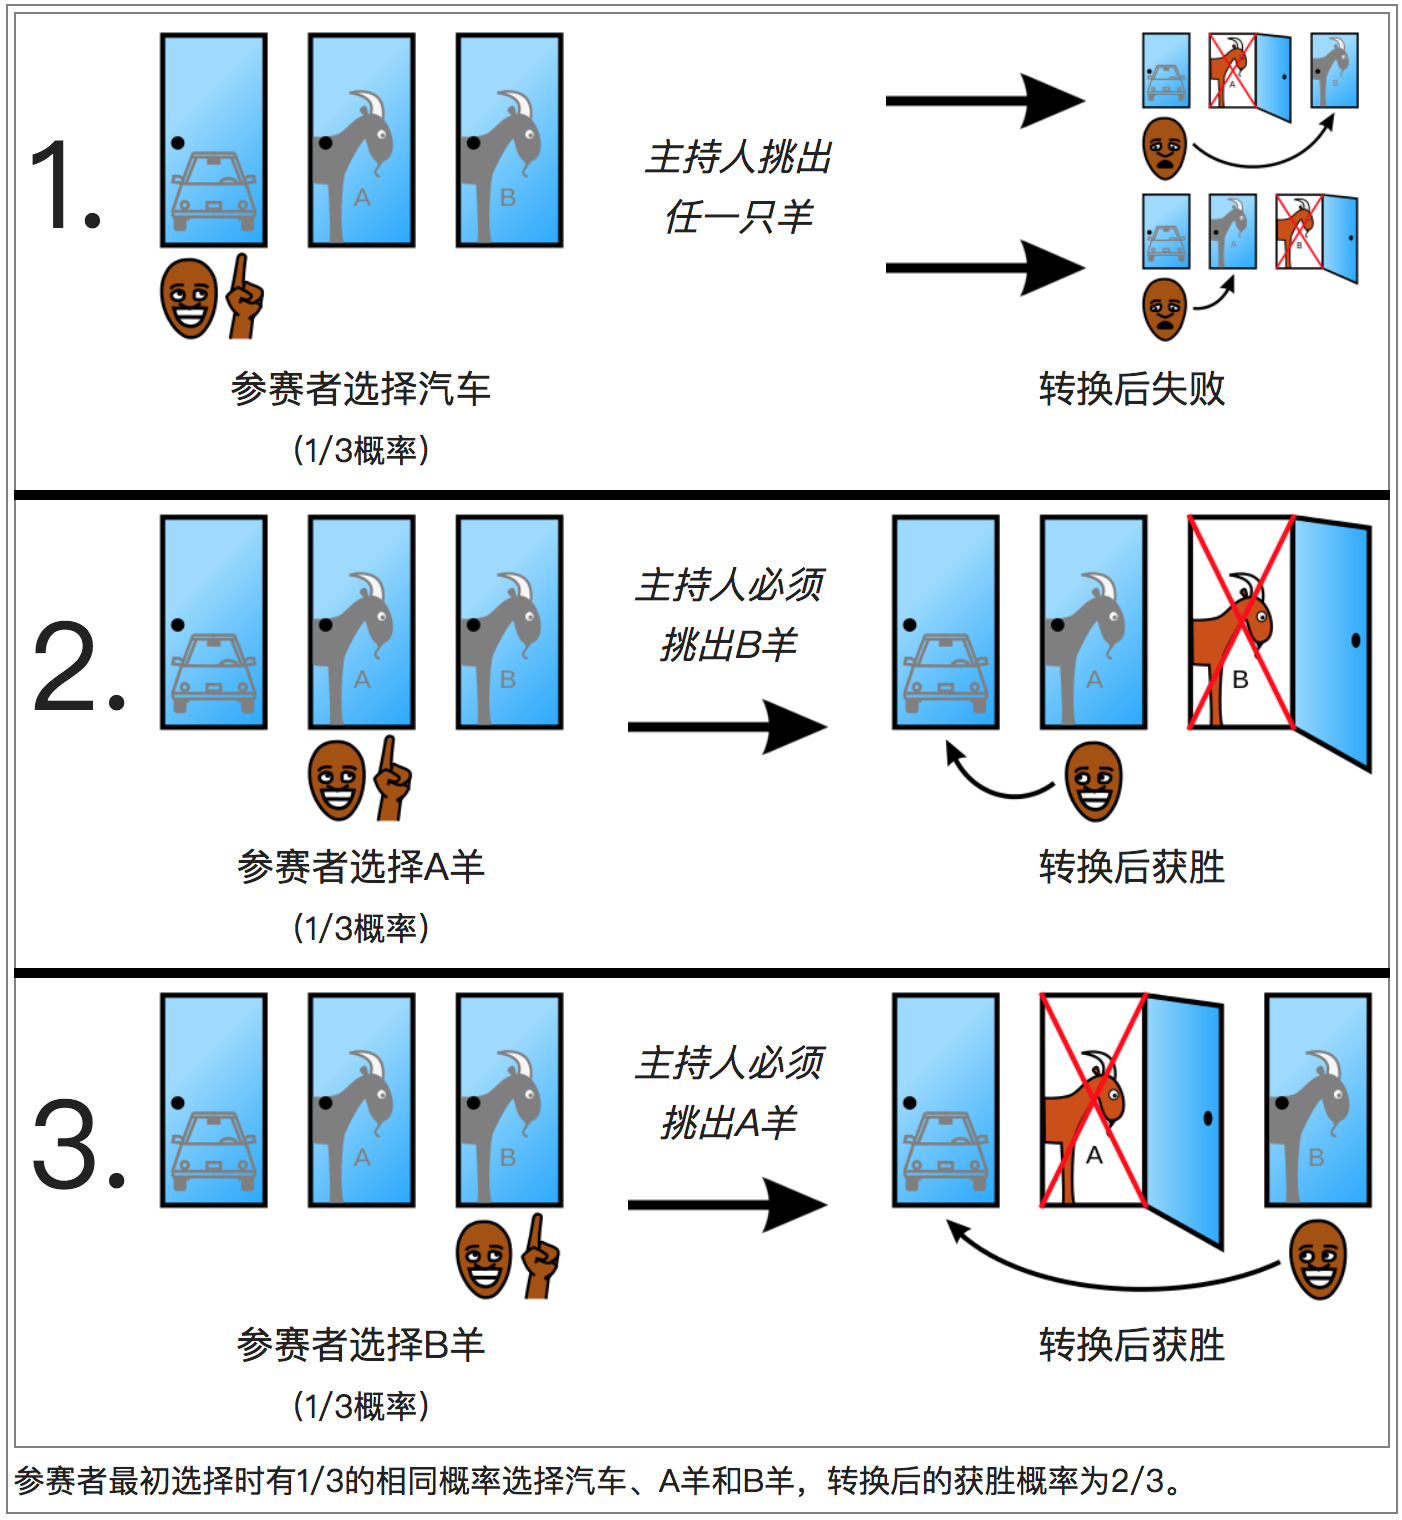
\includegraphics[width=0.5\textwidth]{images/montyhall.png}
	\end{center}
\end{frame}

\subsection{期望}
\begin{frame}
	\frametitle{随机变量与期望}
	\begin{itemize}
		\item \textbf{随机变量}:即将样本点映射到实数域的函数$X:\Omega\rightarrow\mathbb{R}$。
		\item \textbf{期望}:即随机变量在概率意义下的平均值
			\[ \mathbb{E}[X]=\sum_{\omega\in\Omega} X(\omega)P(\omega) \]
			也记作$\mu_X$。
	\end{itemize}

	举个例子,假设抽奖得到一二三等奖和谢谢惠顾的事件分别为$A_1,\ldots,A_4$,其概率分别为$0.01,0.02,0.07,0.9$。那么设随机变量$X$代表抽奖得到的奖金,$X(A_1)=1000,X(A_2)=500,X(A_3)=100,X(A_4)=0$,其期望为
	\[ \mathbb{E}[X] = 1000\times0.01 + 500\times0.02 + 100\times0.07 + 0\times 0.9 = 27 \]
	这意味着抽奖券至少得卖27元。
\end{frame}
\begin{frame}
	\frametitle{期望的性质}
	\begin{itemize}
		\item \textbf{线性性}:对于任意随机变量$X$和$Y$,满足
			\[ \mathbb{E}[\alpha X+\beta Y] = \alpha\mathbb{E}[X] + \beta\mathbb{E}[Y] \]
	\end{itemize}
	期望的线性性是始终成立的,无论两随机变量是否独立。
\end{frame}

\subsection{例题}
\begin{frame}
	\frametitle{例题:矩形粉刷}
	有一块$N\times M$的矩形网格要进行粉刷。每次粉刷会等概率选取两个格子,粉刷以这两个格子为顶点的矩形区域。求经过$K$次粉刷后,至少被刷了一次的格子数的期望。

	$N,M\leq 1000$,$K\leq 100$。
\end{frame}
\begin{frame}
	\frametitle{例题:矩形粉刷}
	我们可以单独求出每个格子在$K$次粉刷之后被粉刷至少一次的概率。由期望的线性性,答案就是每个格子的概率乘以贡献(为1)之和。\pause

	而一个格子在每次粉刷中被刷到的概率是相同的。设其为$x$,那么在$K$次粉刷中被刷到至少一次的概率为$1-(1-x)^k$。

	而这一概率需要根据每个格子的坐标计算,公式从略。
\end{frame}

\begin{frame}
	\frametitle{例题:游走}
	给定一个$N$个点和$M$条边的简单无向图。从$1$号节点出发,每次等概率地随机沿着一条边``游走''到相邻的节点,到$N$号点时结束游走,定义其游走的代价为路程中经过的所有边的编号和(一条边如果被经过多次也要被计算多次)。现在由你来给这些边编号,所有边的编号应该是一个$1\sim M$的排列。请求出游走代价的期望值的最小值。

	$N\leq 500$,$M\leq N^2$。
\end{frame}
\begin{frame}
	\frametitle{例题:游走}
	如果可以求出每条边被经过的期望次数,那么按照期望次数贪心地编号就行了。问题的关键就在于求出期望次数。\pause

	换个角度思考,如果我们能求出每个点被经过的期望次数呢?对于一条边$(a\leftrightarrow b)$,我们经过这条边,要么是从$a$走到$b$,要么是从$b$走到$a$,和其他的点都无关。

	设$D_a$为点$a$的度数,$E_a$为点$a$被经过的期望次数,那么一条边$(a\leftrightarrow b)$被经过的期望次数就是$\frac{E_a}{D_a}+\frac{E_b}{D_b}$。
\end{frame}
\begin{frame}
	\frametitle{例题:游走}
	接下来所求的就是每个点被经过的期望次数。对于每个点我们可以列出一个等式:
	\[ E_a=\sum_{(b\rightarrow a)\in E} \frac{E_b}{D_b} \]

	需要注意几点:
	\begin{itemize}
		\item 题目给的是无向边,这里应该拆成两条有向边处理;
		\item 由于走到$N$号节点就不会再继续游走,所以应该删除从$N$号节点出发的所有有向边;
		\item 由于一开始就处于$1$号节点,所以$1$号点的等式最后还应加上一个常量$1$。
	\end{itemize}
\end{frame}
\begin{frame}
	\frametitle{例题:游走}
	现在我们有了$N$个方程,只需要用高斯消元求解,就可以得出每个节点被经过的期望次数了。

	需要注意的是,由于未知数都是实数,所以可能会存在精度问题。

	另外,根据定义$E_n>0$,但在计算边被经过的期望次数时应当令$E_n=0$。

	复杂度为$O(N^3)$。这一方法也是解决这类问题的较为通用的算法。
\end{frame}
\begin{frame}
	\frametitle{例题:游走}
	我们也可以求出路径的期望长度,即$\sum_x E_x$。这里其实运用了期望的线性性。

	有没有其他做法呢?\pause
	\vspace{1em}

	我们可以设$E_x$表示从$x$走到$n$的期望步数,那么有
	\[ E_a=\sum_{(a\rightarrow b)\in E} \frac{E_b}{D_a} + 1 \]
	特别地,$E_n=0$。

	这个式子与之前的区别在于:枚举的是反边,式尾加了$1$。

	需要注意的是,这里我们是在\textbf{倒推}。主要原因是,倒推时我们可以确定$E_n=0$。而正推的时候$E_1$未必等于$0$,从而无法表示从$1$出发这一信息。
\end{frame}

\begin{frame}
	\frametitle{例题:XOR和路径}
	给定一个$N$个点和$M$条边的有向图(可能存在重边或者自环),每条边有一个非负整数权值。从$1$号节点出发,每次等概率地随机沿着一条边走到相邻的节点,到$N$号点时结束,定义其代价为路程中经过的所有边的权值的异或和(一条边如果被经过多次也要被计算多次)。求出异或和的期望值。

	$N\leq 100$,$M\leq 10000$。
\end{frame}
\begin{frame}
	\frametitle{例题:XOR和路径}
	这道题和上一道题类似,区别就在于这道题求的是异或和,从而无法直接列方程求解。\pause

	注意到异或的一个性质:每一位都互相独立。也就是说,每一位可以分开处理,我们只需要考虑每条边的边权都是$0$或者$1$的图。
\end{frame}
\begin{frame}
	\frametitle{例题:XOR和路径}
	我们使用倒推的方法尝试求解。

	设$E_x$为从$x$号走到$n$的期望代价。如果经过了一条边权为$0$的边,那么代价不会改变。如果经过了一条边权为$1$的边,代价会从$0$变成$1$,从$1$变成$0$,反应到期望上就是会从$E_x$变成$1-E_x$。对前一题的等式稍加修改:
	\[ E_a=\sum_{(a\rightarrow b:w)\in E} \left\{\begin{array}{ll}
		\frac{E_b}{D_a}		& w=0 \\
		\frac{1-E_b}{D_a}	& w=1 \\
	\end{array}\right. \]
	其中$(b\rightarrow a:w)$代表一条从$b$到$a$、权值为$w$的边。
\end{frame}
\begin{frame}
	\frametitle{例题:XOR和路径}
	如果利用线性性正推呢?\pause

	其实也可以。设$E_x^{(1)}$和$E_x^{(0)}$分别代表到达该点时权值分别为$1$和$0$的期望次数。方程类似。
\end{frame}

\begin{frame}
	\frametitle{例题:禁忌}
	有$N$个字符串被称作``禁忌串''。对于一个字符串,将其划分成若干段,如果某段为一个禁忌串,那么就可以造成$1$点``伤害''。一个字符串的``伤害值''就是所有划分方案中最大的总伤害。现在随机生成一个长度为$L$的字符串,求其期望伤害值。

	$N\leq 5$,$L \leq 10^9$,每个禁忌串的长度$\mathit{Len}$不超过$15$。
\end{frame}
\begin{frame}
	\frametitle{例题:禁忌}
	假设我们得到了一个字符串,我们怎么求它的伤害值?\pause

	使用动态规划。设$f[i]$为到第$i$位为止的前缀的最大伤害值,可以列出转移方程:
    \[f[i]=\max_{0\leq j<i}\{f[j]+\mathrm{isTaboo}(j+1,i)\}\]
    其中$\mathrm{isTaboo}(l,r)$代表字串$[l,r]$是否为禁忌串,如果是则为$1$,否则为$0$。计算的时间复杂度为$O(L^2)$。\pause

    不难发现,这个动态规划可以用一个贪心过程来代替:从头开始寻找一个是禁忌串的、且右端点最靠左的子串,然后从找到字串的右端点的右侧的位置再次寻找,直到找不到为止。

    这一过程可以用AC自动机优化到$O(L)$。AC自动机的一个基础应用就是求一个字符串内出现的在字典中的可重叠的单词个数,这里只要稍作修改就可以求出不可重叠的最大个数。
\end{frame}
\begin{frame}
	\frametitle{例题:禁忌}
    如何求期望呢?\pause

    在AC自动机上进行DP。对AC自动机的每个节点设一个状态$f[i][j]$,表示一个长度为$i$的字符串在AC自动机上跑,现在在第$j$个节点处,此时的概率。

    转移时,枚举加入末尾的字符,然后沿着AC自动机的边移动到下一个节点。如果加入字符后会到达终止节点,下一步就应移动到根节点,并增加$1$的伤害。\pause
    
    由于AC自动机的节点数与字符串总长同阶,所以我们可以用矩阵乘法来加速转移。在处理终止节点增加的伤害时有一个比较巧妙的方法:设一个虚拟节点$0$,当加入字符到达终止节点时,向根节点转移,同时也向$0$号节点转移。这样$0$号节点的期望伤害就会是答案了。
    
    整个算法的时间复杂度为$O((N\cdot\mathit{Len})^3 \log L)$。
\end{frame}


\appendix
\section{结语}
\begin{frame}
	\frametitle{Fin.}
	\centering
	\LARGE
	谢谢大家!欢迎课后交流。
\end{frame}

\section{证明}
\subsection{矩阵树定理:最后一步的证明思路}
\begin{frame}
	\frametitle{证明思路}
	\label{appendix:mtt}
	当图不连通时,可以将$\mathbf{F}_S$写成$\mathrm{diag}(\mathbf{M_1},\mathbf{M_2})$的形式,其中$\mathbf{M_2}$每列包含恰好一个$1$和$-1$。那么$(0,\ldots,0,1,\ldots,1)^\top$是其特征向量,对应特征值为$0$,故$\det{\mathbf{F}_S}=\det{\mathbf{M_1}}\det{\mathbf{M_2}}=0$。

	当图非树时,必然含有一个环,而因为图只包含$n-1$条边,必然不连通。故此时$\det{\mathbf{F}_S}=0$。

	当图是一棵树时,可以归纳证明$\det{\mathbf{F}_S}=\pm 1$。
\end{frame}


\end{document}
